\section{Results and Discussion}

For the results of this Project, we represented the retrieved topic model in plots. For one we 
used a simple plot package, ggplot in R, to represent every of Lovecraft’s works in chronological 
order with their distribution of the topics. We also used the R package LDAvis to show correlations 
between the topics and use an interactive interface to see the importance of relevant terms with 
respect to a topic. The resulting topics are as follows:

\begin{enumerate}
    \itemsep0em
    \item thing, time, feel, mind, life
    \item thing, horror, eye, black, sound
    \item dream, city, day, night, strange
    \item room, door, hand, floor, window
    \item place, wall, stone, vast, foot
    \item west, specimen, work, lake, body
    \item letter, curwen, time, late, charles
    \item street, house, hill, place, town
    \item family, child, son, home, time
    \item thing, folk, time, good, obed
    \item voice, sound, begin, word, time
    \item tomb, night, fear, thing, remain
    \item land, city, sea, dream, water
    \item thing, night, place, talk, people
    \item carter, ghoul, cat, night-gaunts, ship
\end{enumerate}

\begin{figure}[ht]
    \centering
    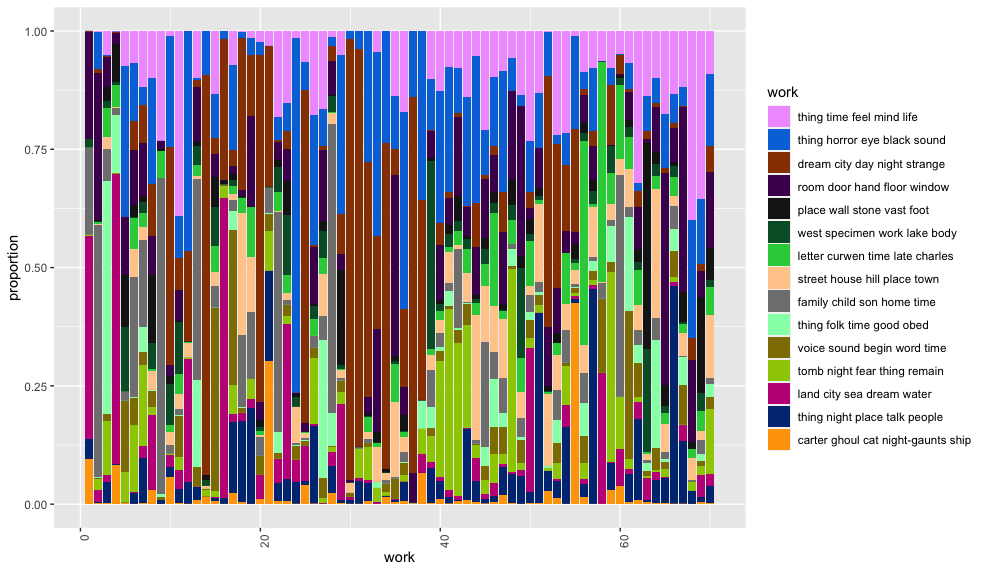
\includegraphics[width=1\textwidth]{/Users/ferriskleier/PECK/DigitalHumanities/Lovecraft_TopicModel/Project/images/plot.png}
    \caption{The plot assigning the proportion of a topic to each story of Lovecraft}
    \label{fig:mesh1}
\end{figure}

Figure 1 shows the bar chart we created to plot every of Lovecraft’s stories in chronological order 
with the percentage of the topic they share. On the x-axis, you can see the number of the story. 
Keep in mind that we used the date Lovecraft wrote the story and changed unspecified dates like just 
a year to the January of that year. For the enumeration of his works to compare to this figure, see 
stories\_list.txt. On the y-axis, you can see the distribution in percentage. Each bar corresponds to 
one work and the percentage of a topic across each of the topics in that work. The order for each 
topic per entry is the same, it’s not ordered by percentage but by topic. On the right-hand side, you 
can find the colors for each topic, pink being topic 01 consisting of the words ‘thing, time, feel, 
mind, life’.\\

The bar chart clearly shows that some topics dominate a story and others have a fairly distributed 
amount of topics. For example, the first topic in pink is highly present in some works. For 
work 55, ‘The Dream Quest of Unknown Kadath’ (written 1927) one can see that topic 15 is highly 
present, which satisfies the expectation because it is a fairly long work with a unique setting 
and motif. Another example is work 63, ‘At the Mountains of Madness’ (written 1931), the topics 
5 and 6 are more present than in any other work, which again satisfies the expectation for this 
work being unique in the antarctic setting and length. The bar chart also shows batches of topics 
for several time frames, like his works 30 to 38 which are dominated by topic 3. After reviewing 
the topic distribution for every work, we were very satisfied with the results and decided to use 
this resulting topic model for further examination.\\

To put this into context with Lovecraft’s personal life, we took several events that may have had 
a significant influence on him and checked for the topics of that time. We reviewed ‘An Epicure in 
the Terrible’ (Edited by David E. Schultz and S.T. Joshi) which is a perfect collection of essays 
by different authors regarding Lovecraft’s life. Topic 2 being blue clearly shows the time Lovecraft 
began to write the ‘Dream Cycle’, since the topics correlate well with the stories. For work 10, 
‘Polaris’ (written 1918), and work 14, ‘The White Ship’ (written 1919), one can see the high share 
of topic 3, which just continues for later stories in the dream cycle as well. This is due to the 
fact that around this time, Lovecraft met Lord Dunsany, who Lovecraft admired and who heavily 
influenced his early works which led to the dream cycle. For the works 24 (‘Nyarlathotep’, 
written 1920), 26 (‘From Beyond’, written 1920), and 29 (‘The Nameless City’, written 1921) 
topic 2 is highly present and these works mark the first shift in Lovecraft’s writings towards 
cosmic horror, which later caused the works of the ‘Cthulhu Mythos’. Starting from work 30, ‘The 
Quest of Iranon’ (written 1921), topic 3 dominates parts of his writings. Topic 3 is a good indicator 
for writings covering the dream cycle, which matches the works. The first interesting correlation 
between Lovecraft’s personal life and the graph can be seen starting from work 33, ‘The Outsider’ 
(written 1921), with topic 2 (blue) having a great share for some works and before. This may relate 
to the death of his mother in May 1921. Not only did he not write for a short period, but topic 2 
consists of the keywords ‘thing, horror, eye, black, sound’ which suggests a coping to his mother’s 
death as well as the time before may having an impact on this topic as well because she was admitted 
to a hospital. Lovecraft moved to Brooklyn in 1922 and married his wife, Sonia Haft Greene, which 
can be seen in a clear shift in topics during the time around work 39 and following, putting a break 
on the dream cycle and prompting topic 12 to be more present. Topic 12 ends being more present starting 
from work 44, ‘The Festival’ (written October 1923). That’s interesting because he did also write just 
one story for almost two years during that time, which goes in hand with his marriage and time in New 
York. Lovecraft started writing again when in 1925 he moved to Red Hook, Brooklyn, living alone 
because his wife worked somewhere else. It is known that Lovecraft despised Red Hook and was 
negatively standing against minorities that lived there. The only observable difference is, that 
topics 4, 5, and 9 started to have a stable share starting from that time. This started with his 
first story after the break ‘The Horror at Red Hook’ (written 1925) which strongly suggests his 
cope with living there. The next observable pattern begins with work 52, ‘The Strange High House 
in the Mist’ (written 1926), which is represented with a higher amount of topic 3 being the topic 
that indicates the continuation of the dream cycle. This is very interesting, because Lovecraft 
moved back to Providence in April 1926, resulting from his growing homesickness and that he became 
increasingly depressed by his isolation and the masses of “foreigners” in the city. The observation 
of topic 3 being more present again due to the continuing dream cycle indicates this. Another 
interesting correlation with Lovecraft’s stay in Brooklyn comes from topic 13. This topic covers 
terms like ‘sea’ and ‘water’ that are somewhat lacking during his time away from Providence (1922 
to 1926, work 37 to 49). This comes from the fact that Lovecraft was inspired by Providence and 
the nearby sea, though Brooklyn was close to the sea too, it was the city that influenced Lovecraft’s 
themes at that time. For ‘The Dream Quest of Unknown Kadath’ (work 55), it’s probably the most 
important work of the dream cycle and covers the fictional character Randolph Carter, who was 
supposedly an alter ego of Lovecraft as mentioned earlier. The graph also suggests a lower share 
of the first topic during the timeframe for the works covered by that topic, work 56-61 from spring 
1927 to 1930. This correlates to the fact that he divorced in 1929 and there may have been first 
signs of a shift in themes and motifs caused by unknown problems in his and Greene’s relationship 
prior to the divorce. Topic 2 is present in some of the last works again as well as topic 1 having 
a higher share starting at work 62, ‘The Thing on the Doorstep’, which was written in the summer of 
1930. This and the higher share of topic 4 starting from work 65 (‘Dreams in the Witch House’, written 
1932) indicate an observable shift in topics following a break from writing because of the death of 
his aunt Mrs. Clark in 1932 and moving with his other aunt Mrs. Gamwell into small quarters in 
Providence. He was very close with aunt Mrs. Clark and her death could be represented in the shift 
starting at work 65 where topics 4 and 14 become highly present and topic 1 having a noticeably 
higher share from work 68. Another explanation for this mix of topics during the last years could 
be that Lovecraft had a hard time selling his longer stories and concentrated on ghostwriting and 
non-fiction, resulting in the fictional works he wrote being less frequent but longer and more 
focussed on different topics.\\

\begin{figure}[ht]
    \centering
    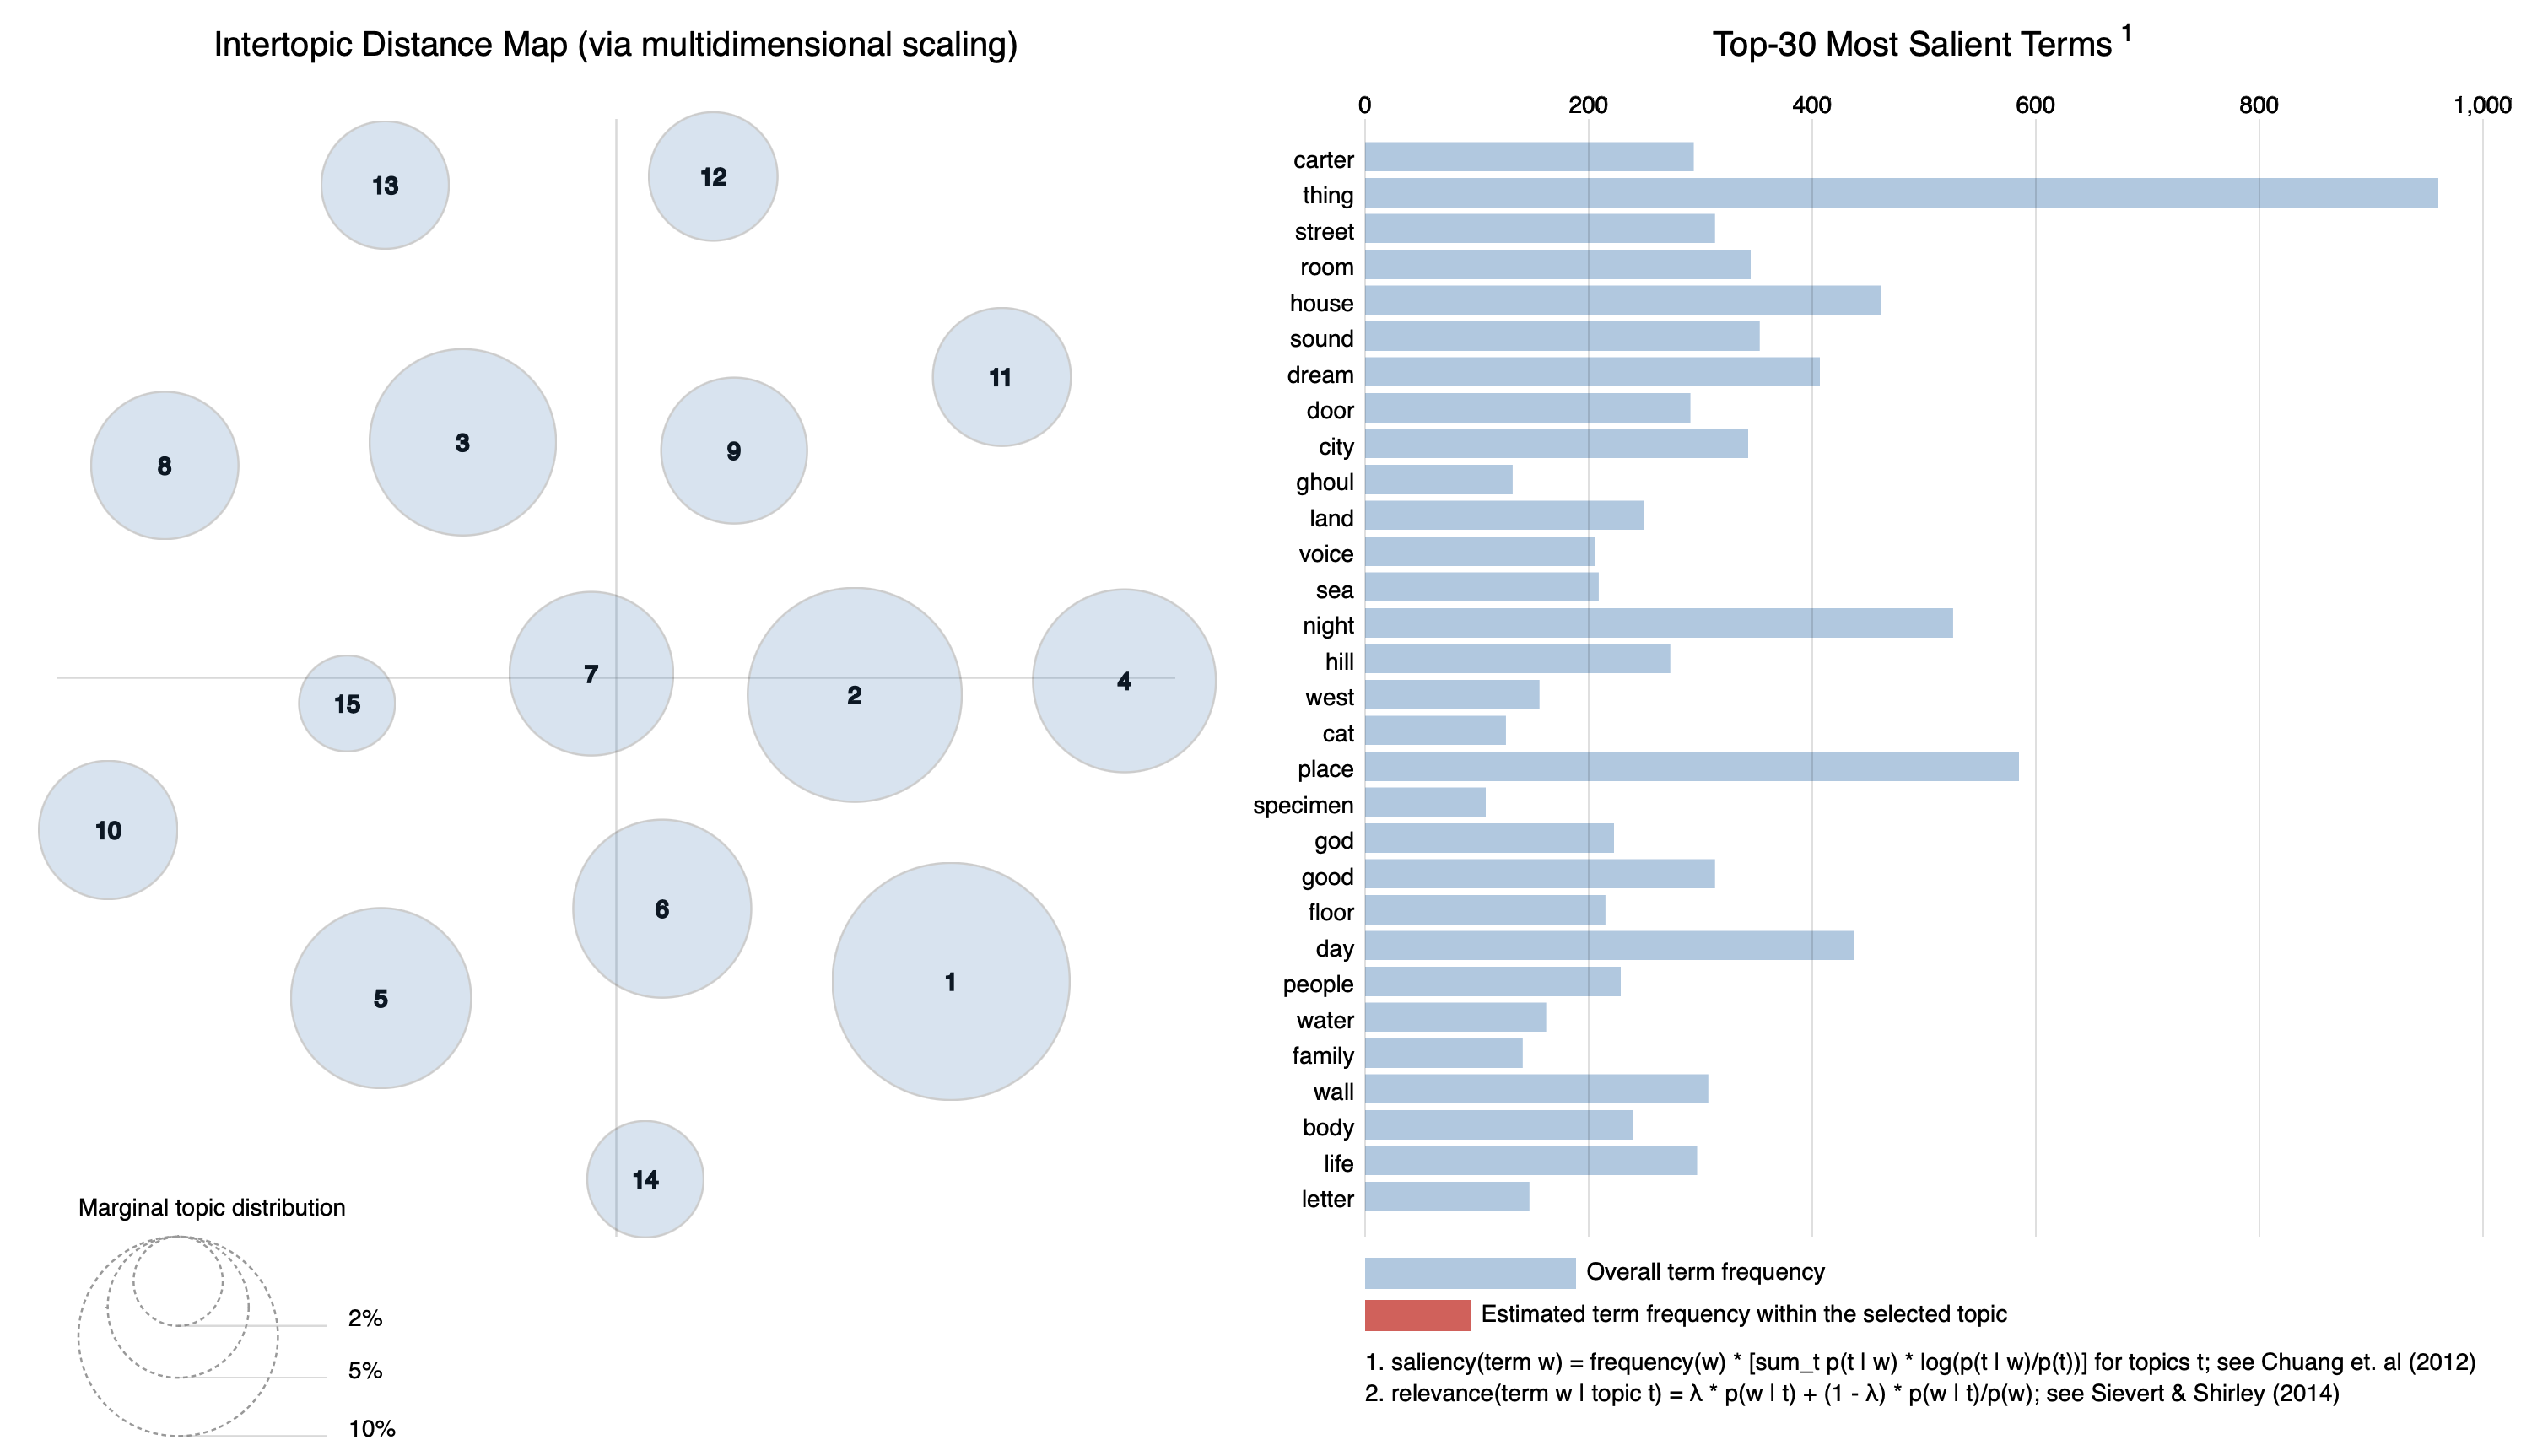
\includegraphics[width=1\textwidth]{/Users/ferriskleier/PECK/DigitalHumanities/Lovecraft_TopicModel/Project/images/ldavis_model.png}
    \caption{LDAvis results}
    \label{fig:mesh2}
\end{figure}

\begin{figure}[p]
    \centering
    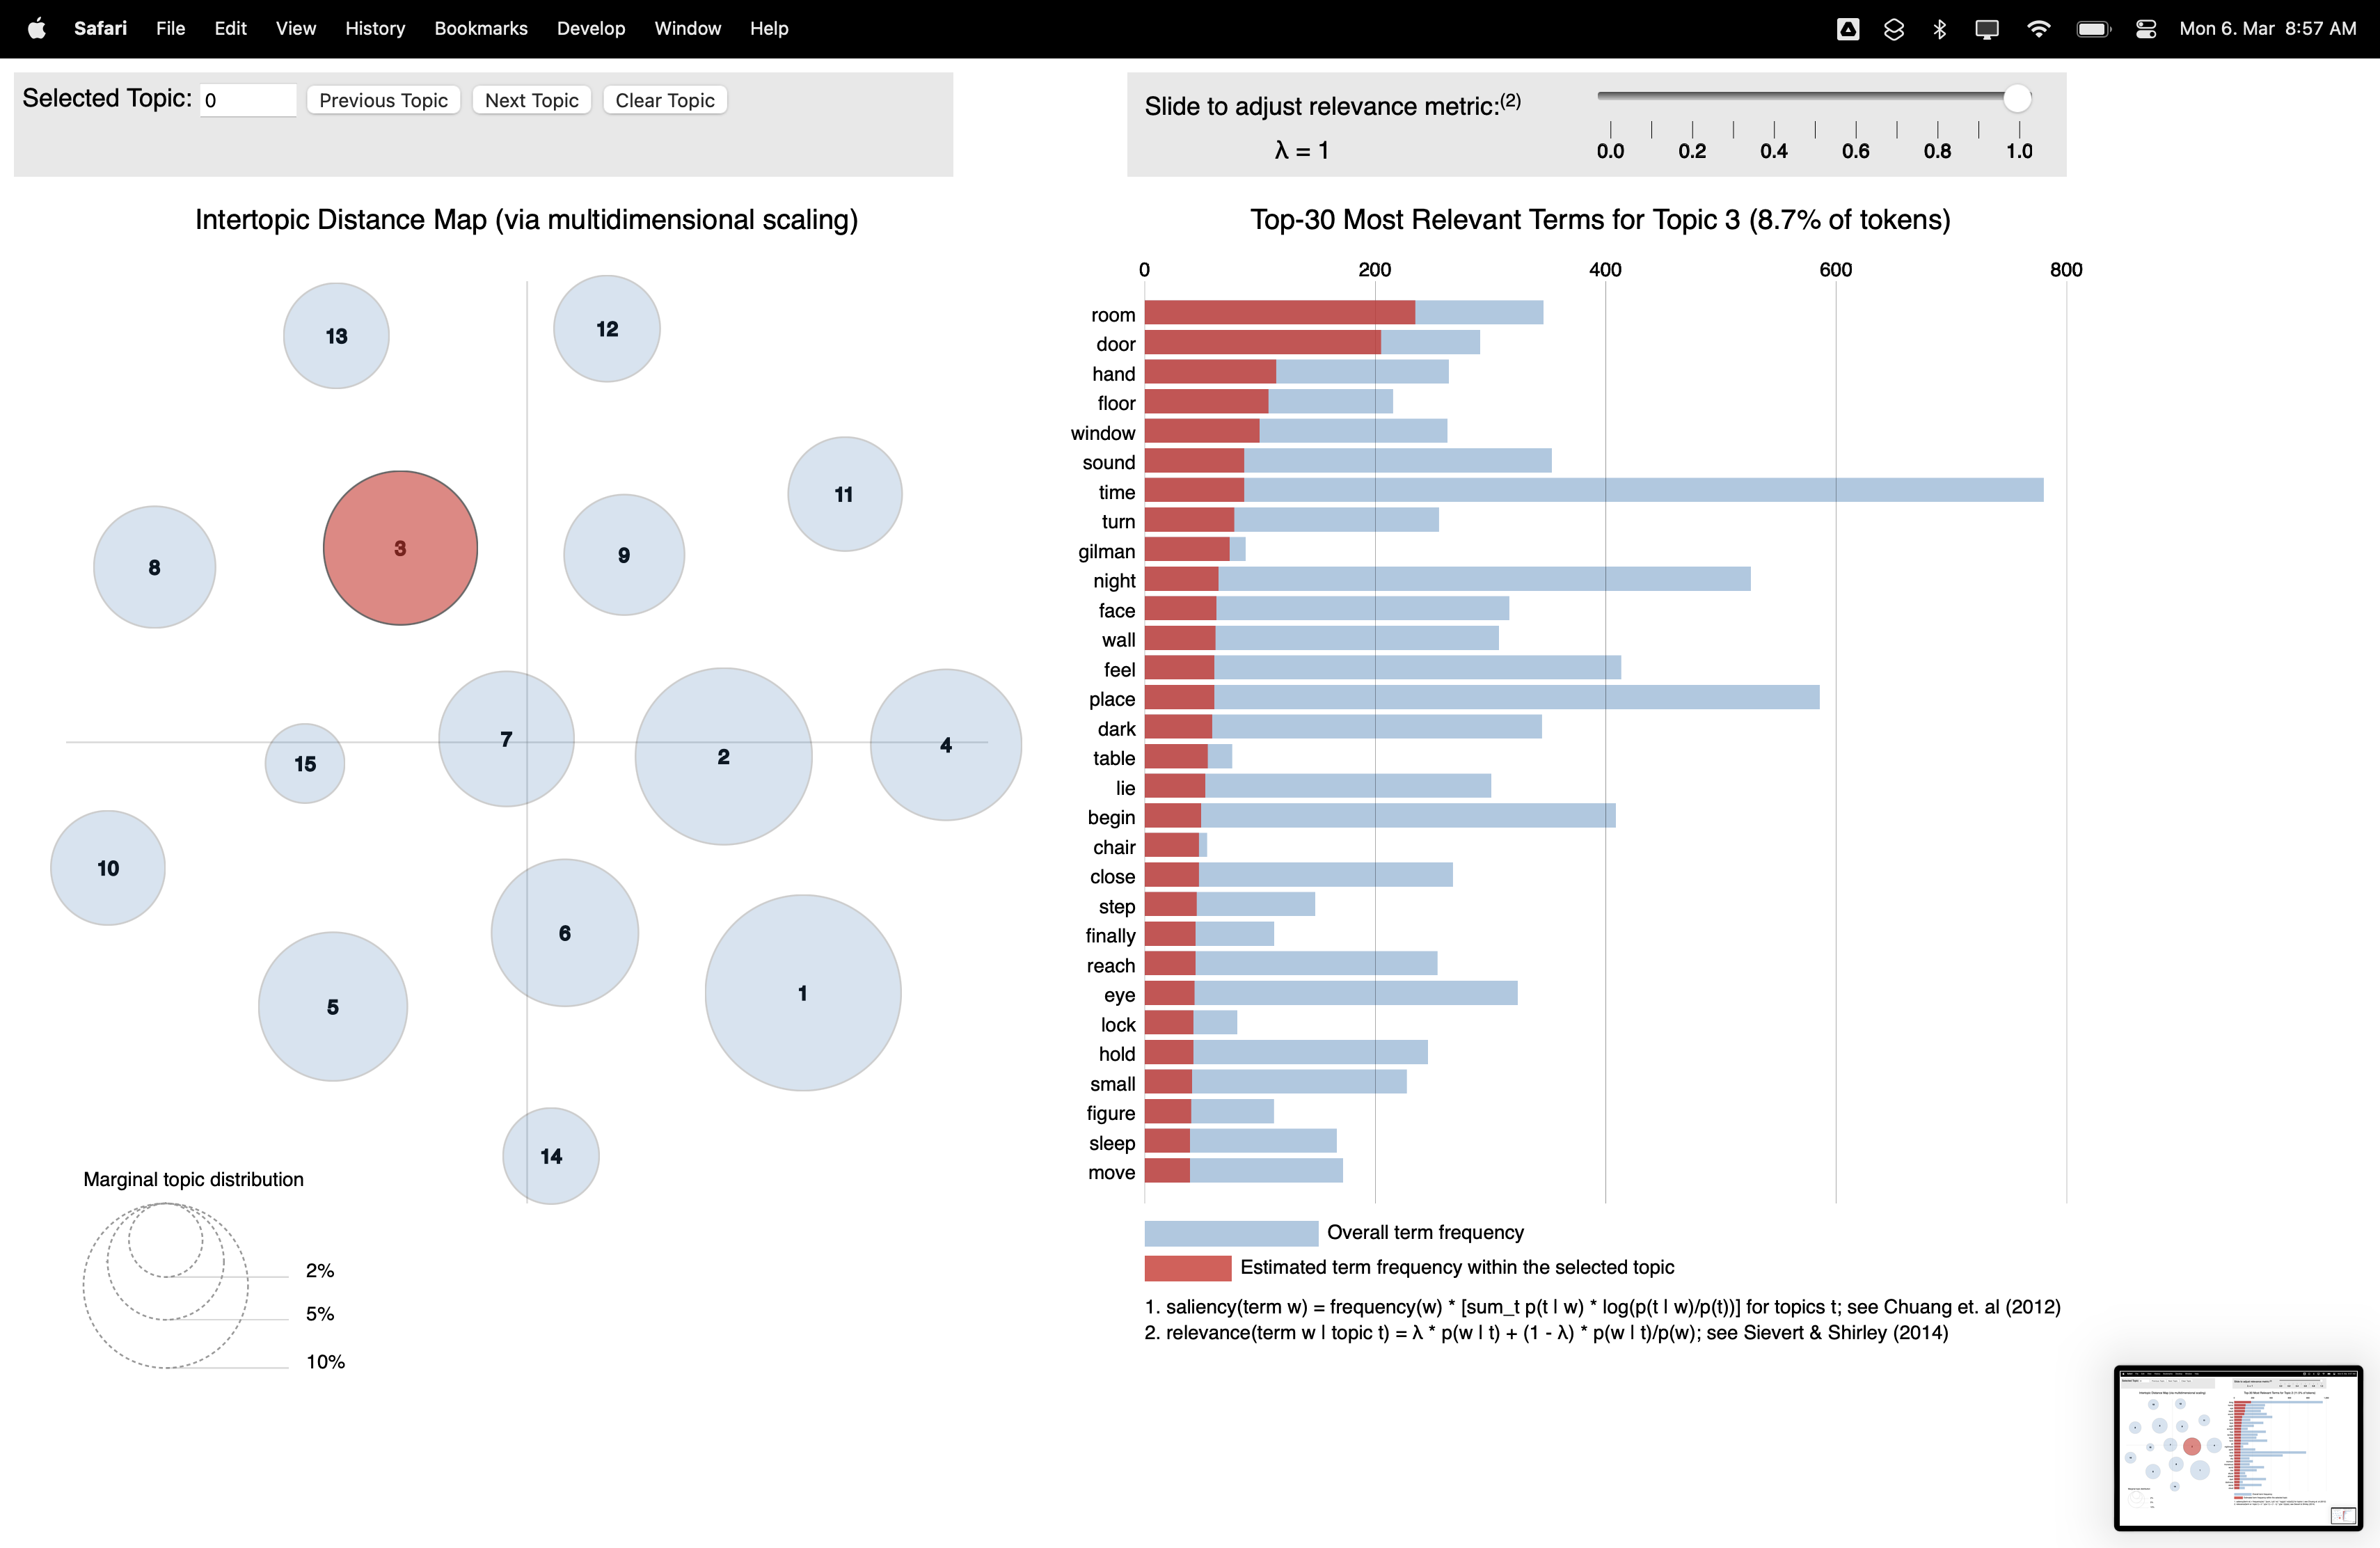
\includegraphics[width=1\textwidth]{/Users/ferriskleier/PECK/DigitalHumanities/Lovecraft_TopicModel/results/LDAvis_lambda-1/ldavis_L-1_03.png}
    \caption{LDAvis results, selected topic 3, $\lambda=1.0$}
    \label{fig:mesh3}
\end{figure}

\begin{figure}[p]
    \centering
    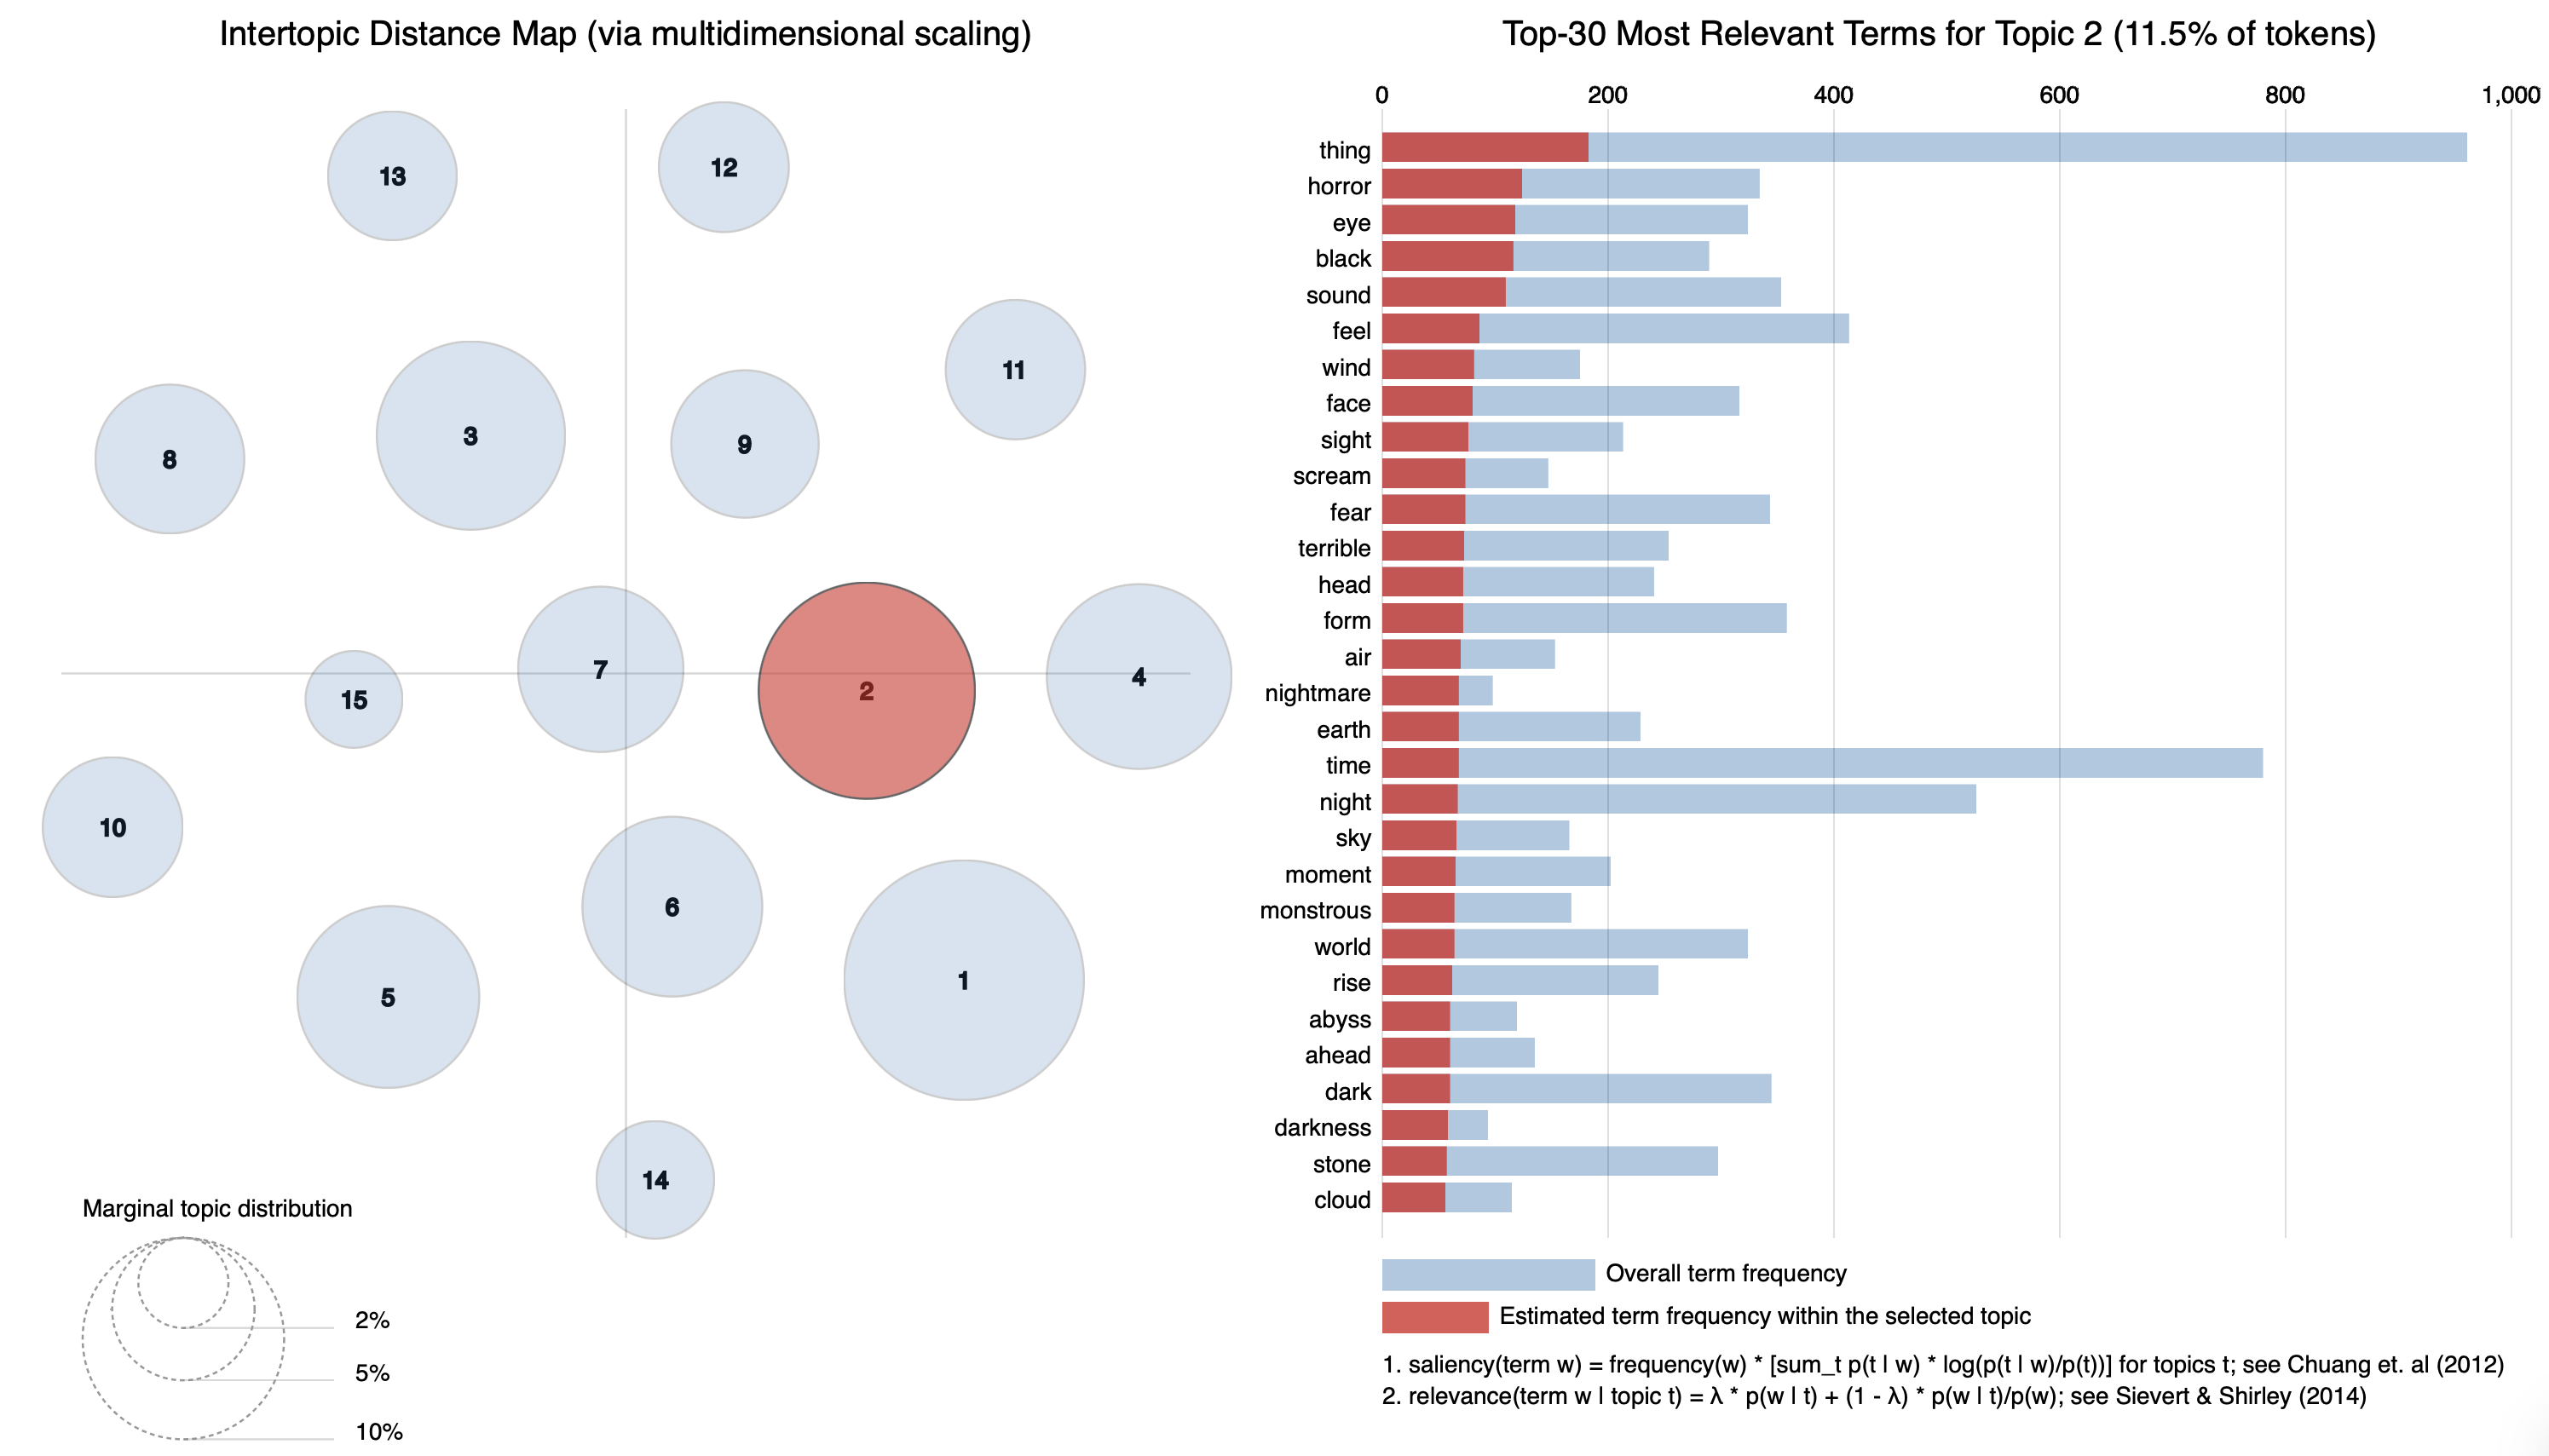
\includegraphics[width=1\textwidth]{/Users/ferriskleier/PECK/DigitalHumanities/Lovecraft_TopicModel/results/LDAvis_lambda-1/ldavis_L-1_02.png}
    \caption{LDAvis results, selected topic 2, $\lambda=1.0$}
    \label{fig:mesh4}
\end{figure}

We also used the R library LDAvis to find correlations between these topics or terms that are heavily 
linked to them. Figure 2 shows the resulting web interface from the topic model we got. The frequency 
of terms is shown on the right side of the plot. The plot represents each topic according to its 
importance within the topic model. The larger the circle, the more important this topic is. The use of 
LDAvis comes in convenient when we click on one of these circles representing a topic. As you can see 
in figure 3, the terms in relation to topic 3 are represented on the right-hand side. For this example, 
we can see that the words room and door are strongly connected to the other terms in that topic. There 
is also a slider to adjust the value for Lambda, which gives less relevant but more frequent terms in 
connection with the topic if Lambda is lower.\\

In context to Lovecraft’s life and insights from the first plot in figure 1, we can focus on some 
topics around already mentioned events. The first is the beginning of the dream cycle in 1920, covered 
by topic 3. As expected we can find a lot of terms relating to the topic of the dream cycle like room, 
sound, night, dark, and time. Stories around the dream cycle are typically not dreams but protagonists 
exploring otherworldly places. That way works 30 and 31 (‘The Quest of Iranon’ and ‘Ex Oblivione’) can 
be described using these relevant terms. One common share across these relevant terms for topic 3 is a 
vague description of the places, feelings, and situations it takes place in, matching Lovecraft’s 
writing of most of the works from the dream cycle according to dreams he had himself.\\



As seen in figure 4, Topic 2, which is associated with the time around his mother’s death, is 
connected to matching terms like horror, fear, terrible, or nightmare. This undermines our expectation 
that topic 2, though also present in earlier works, becomes more present because of his mother’s death 
and yields a stable share for some time.\\

\begin{figure}[p]
    \centering
    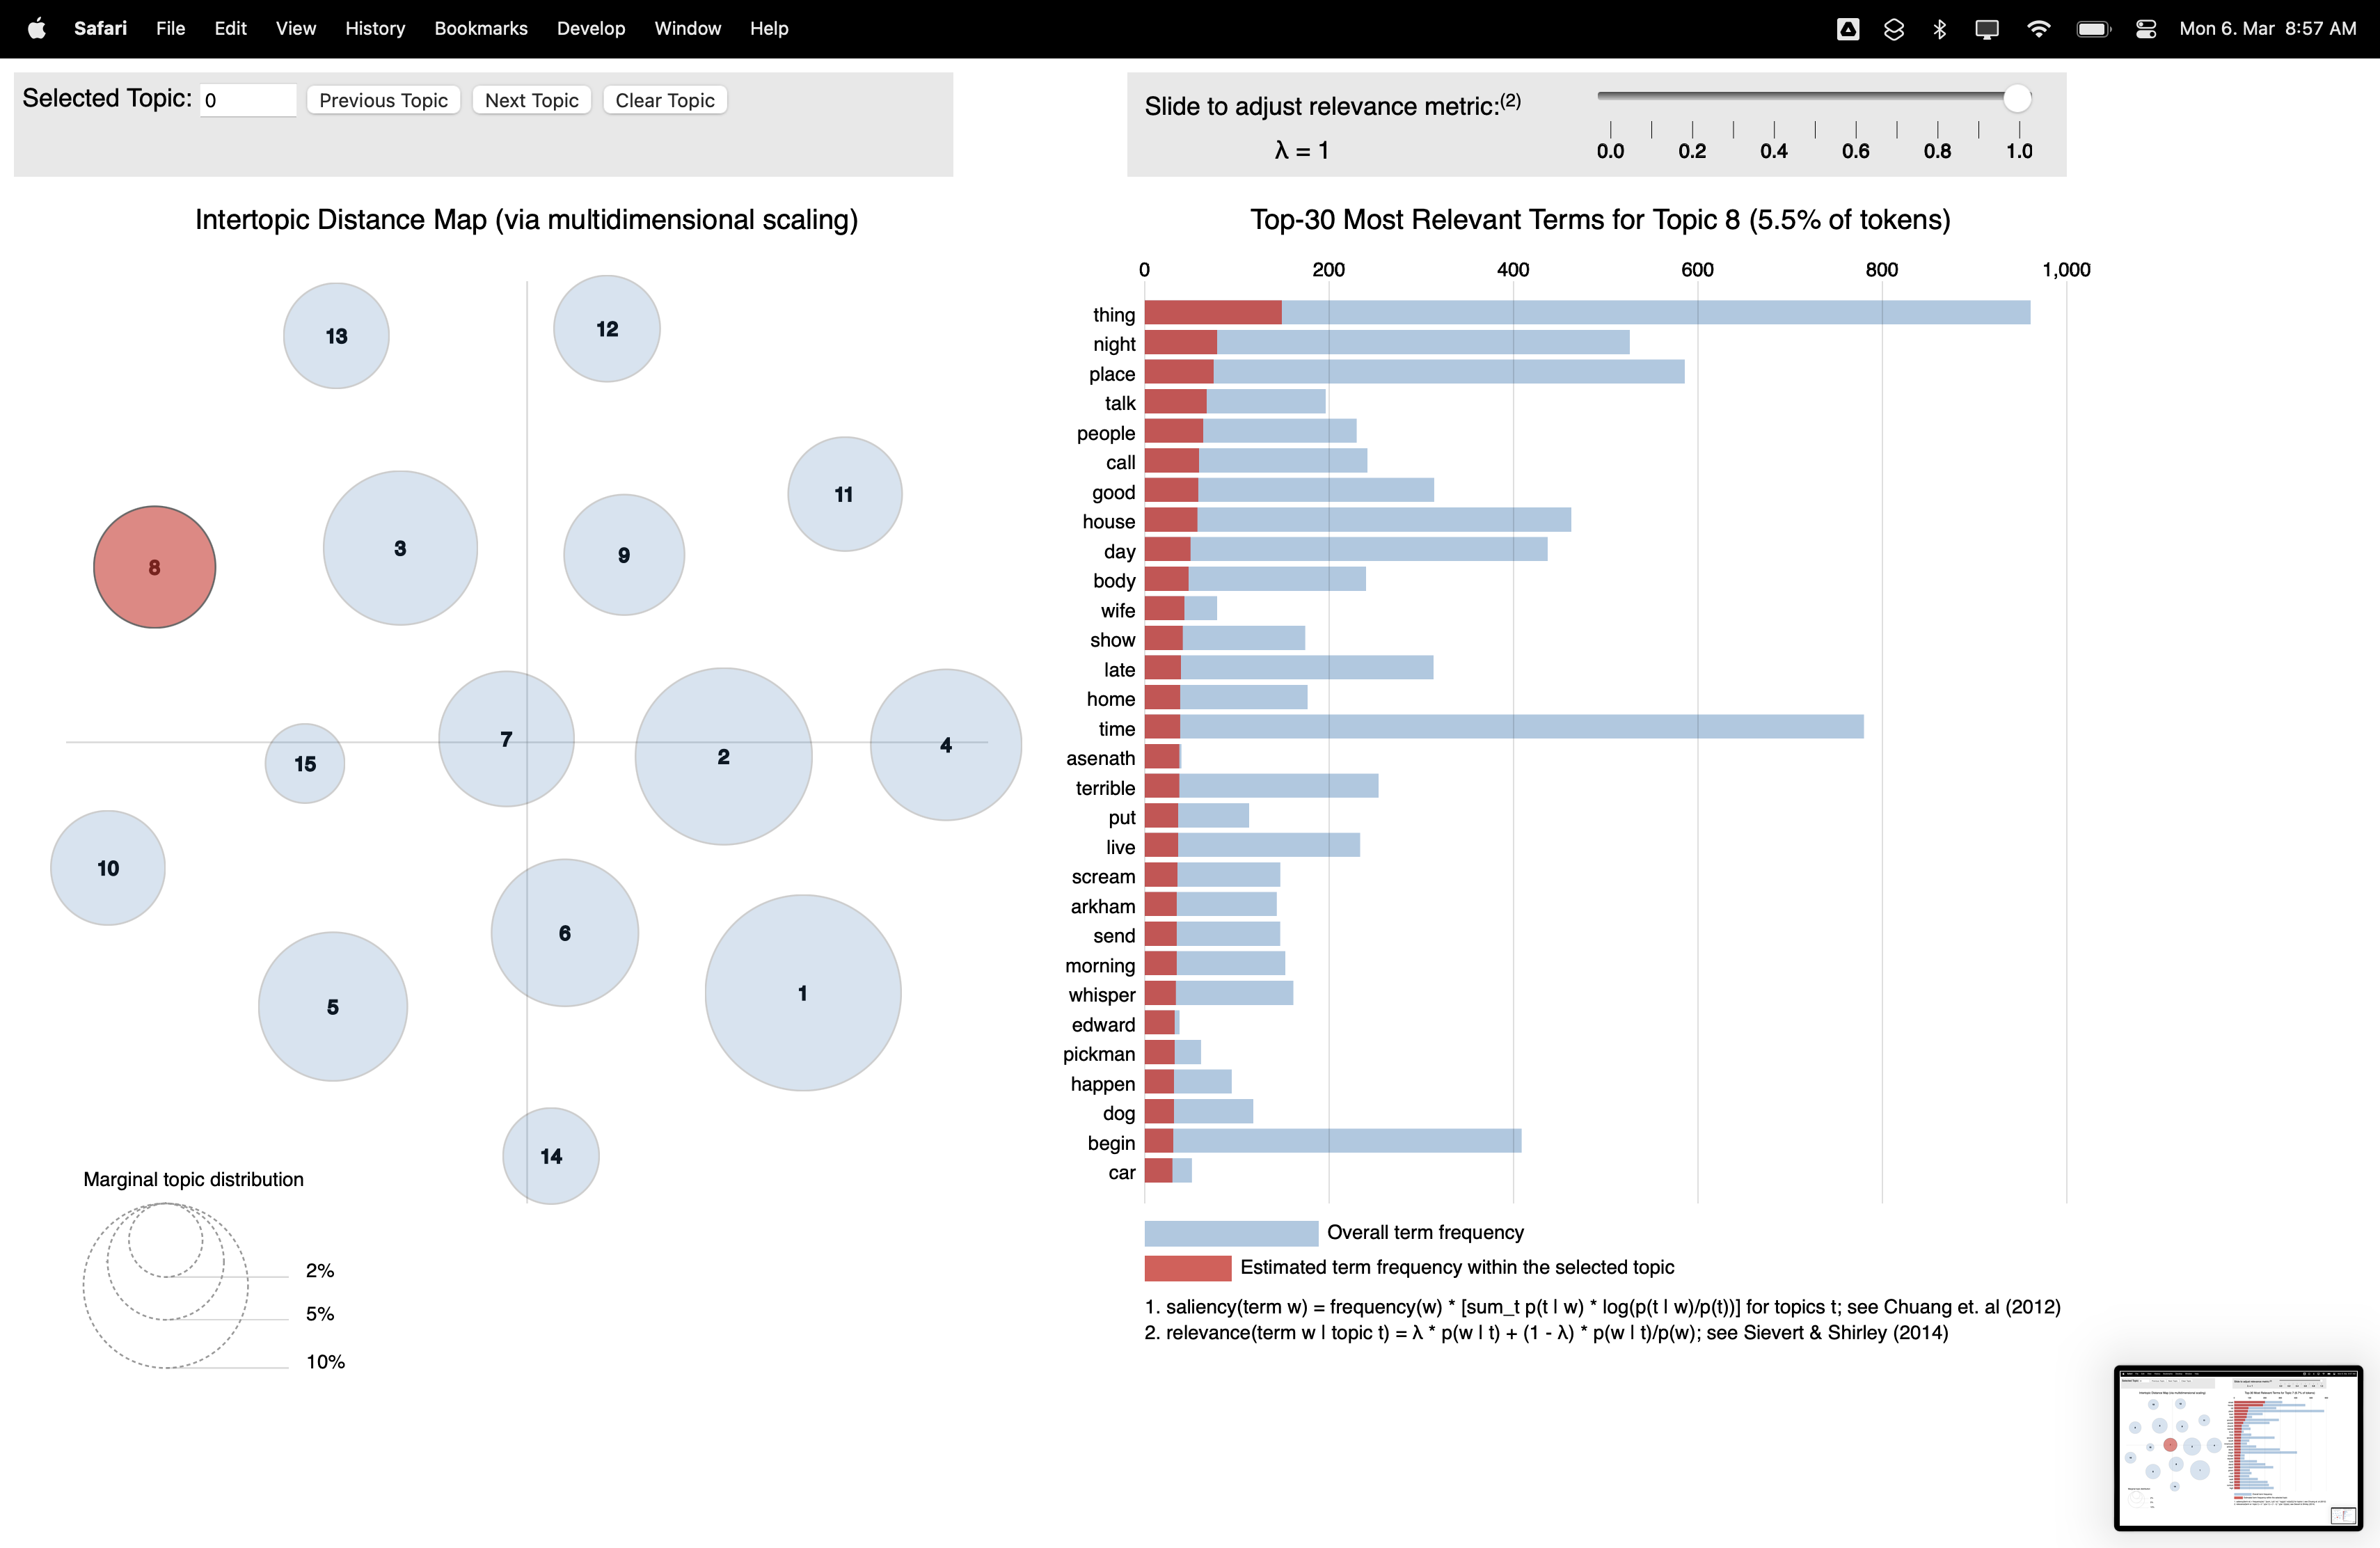
\includegraphics[width=0.49\textwidth]{/Users/ferriskleier/PECK/DigitalHumanities/Lovecraft_TopicModel/Project/images/ldavis_L-1_08.png}
    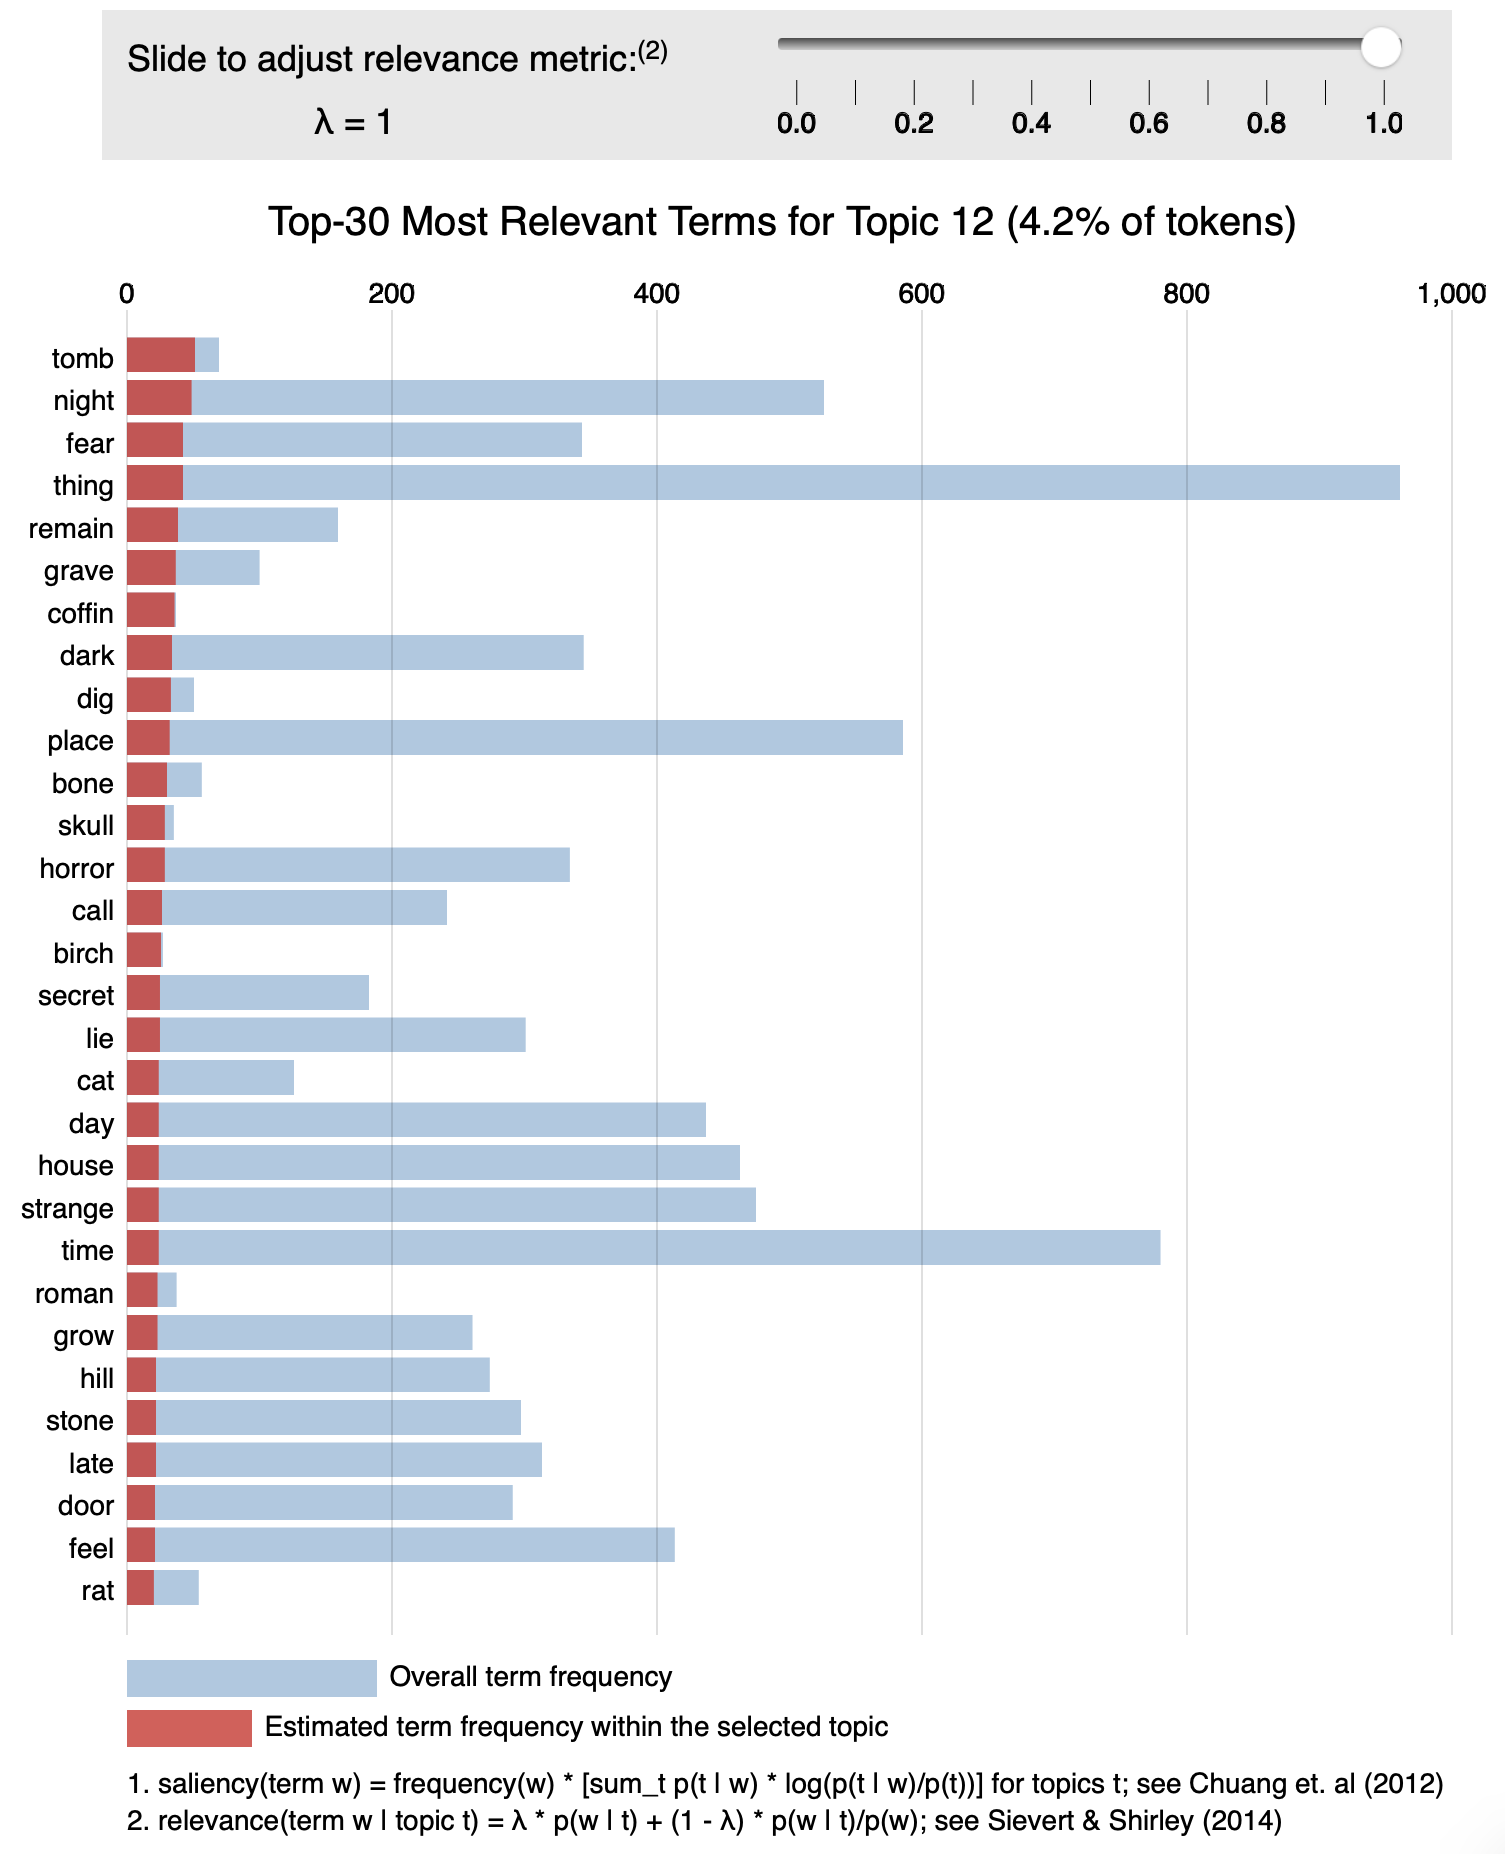
\includegraphics[width=0.49\textwidth]{/Users/ferriskleier/PECK/DigitalHumanities/Lovecraft_TopicModel/Project/images/ldavis_L-1_12.png}
    \caption{LDAvis results, selected topic 8 and 12, $\lambda=1.0$}
    \label{fig:mesh5}
\end{figure}

\begin{figure}[p]
    \centering
    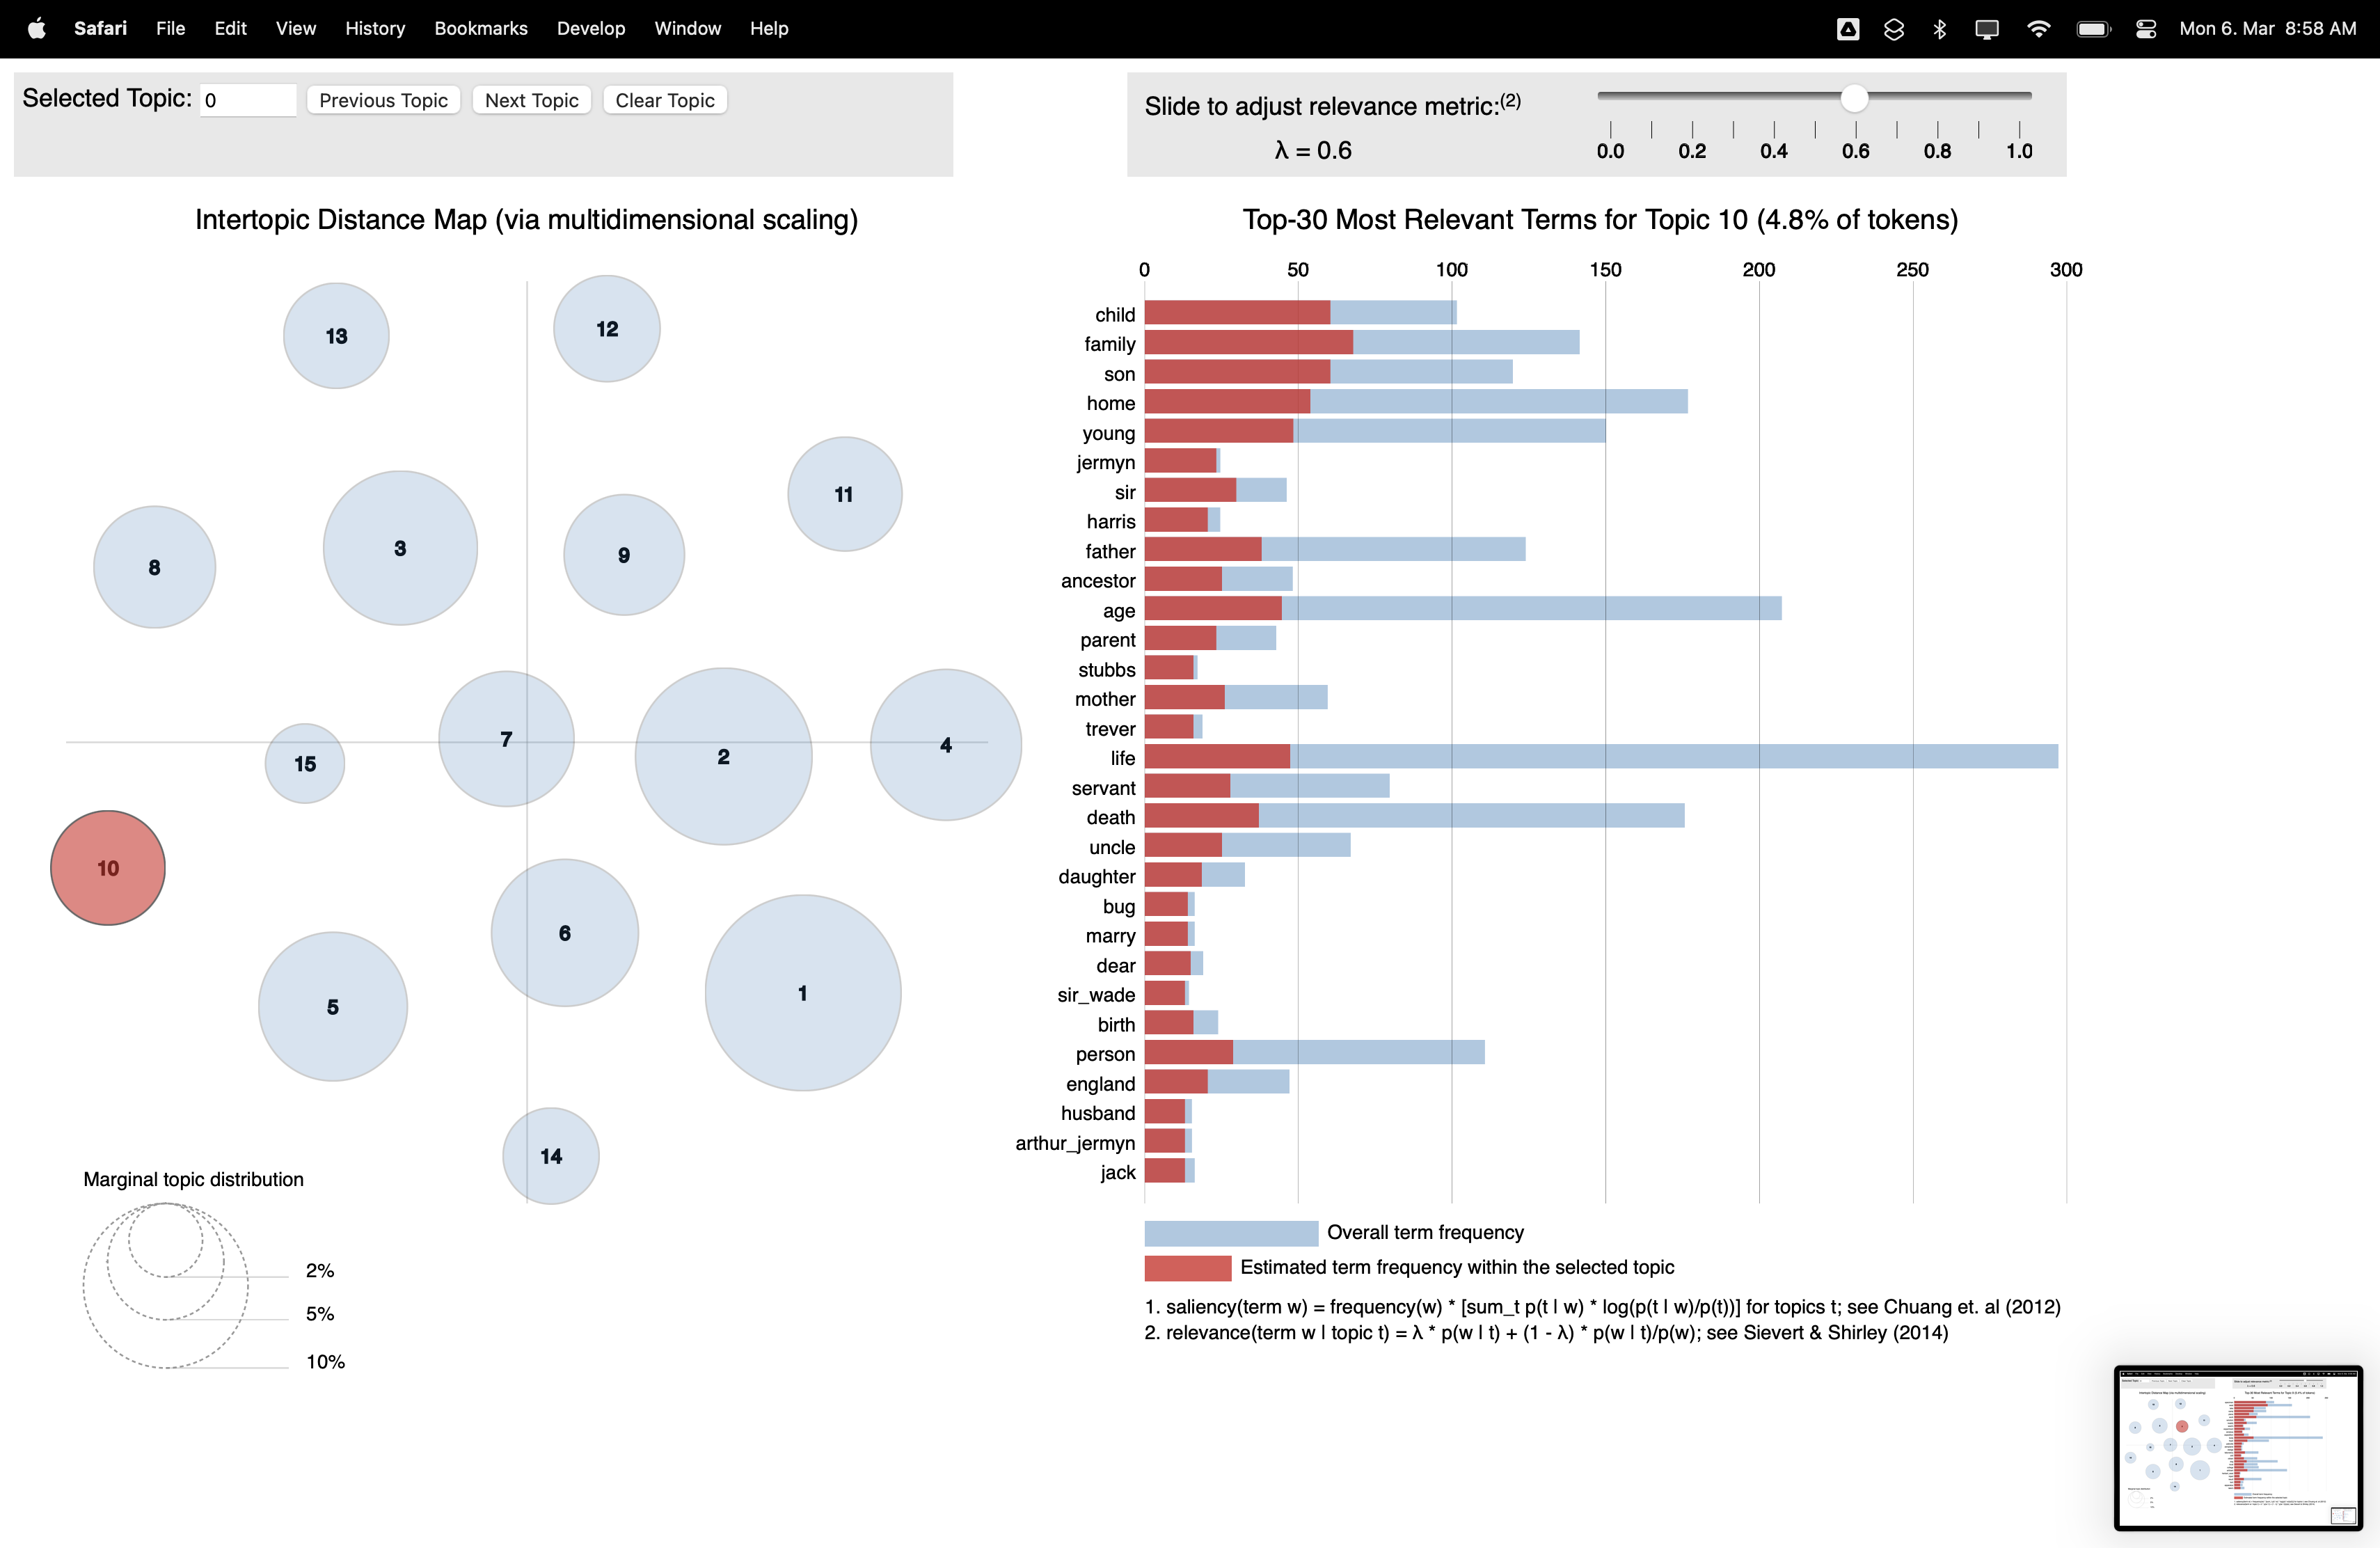
\includegraphics[width=1\textwidth]{/Users/ferriskleier/PECK/DigitalHumanities/Lovecraft_TopicModel/results/LDAvis_lambda-06/10.png}
    \caption{LDAvis results, selected topic 10, $\lambda=0.6$}
    \label{fig:mesh6}
\end{figure}

\begin{figure}[ht]
    \centering
    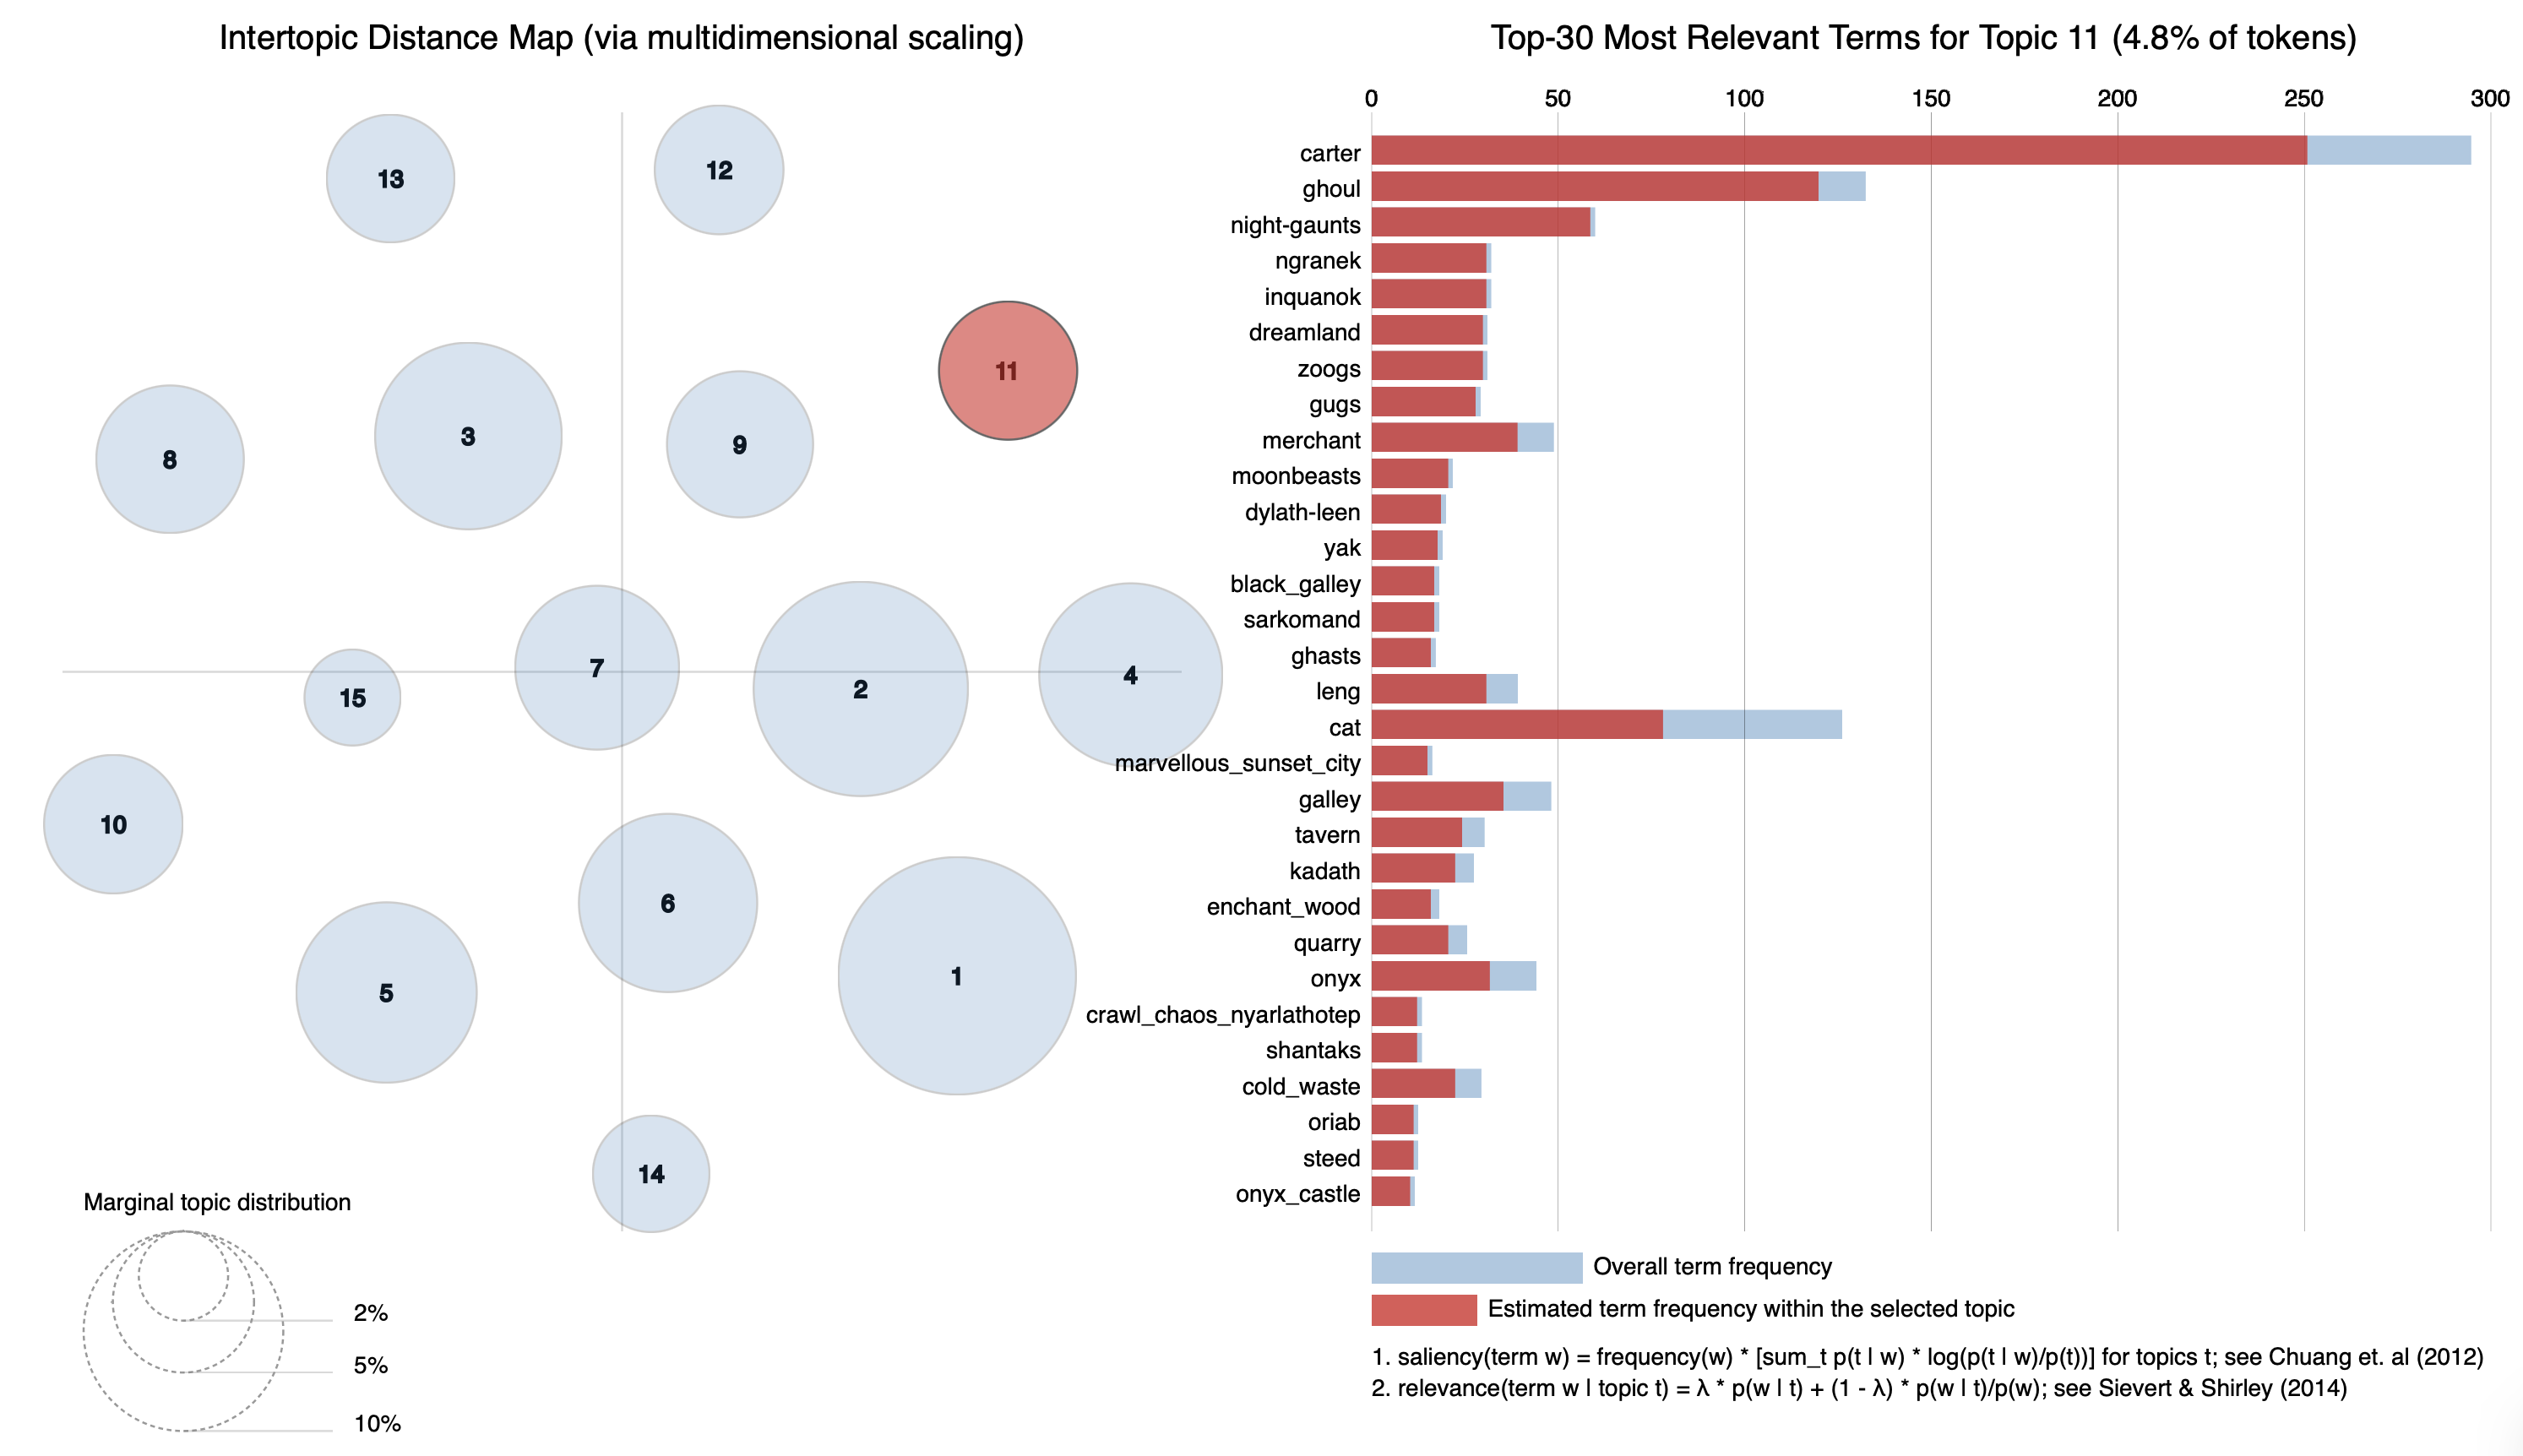
\includegraphics[width=1\textwidth]{/Users/ferriskleier/PECK/DigitalHumanities/Lovecraft_TopicModel/results/LDAvis_lambda-02/11.png}
    \caption{LDAvis results, selected topic 11, $\lambda=0.2$}
    \label{fig:mesh7}
\end{figure}

In figures 5 we can see the relevant terms for topics 8 and 12, which match closest to his stay 
in Brooklyn, cover place, people, wife, fear, and home. That is the most interesting insight because 
as we have seen in figure 1 one can find patterns in the time frames when he moved to Brooklyn and 
back to Providence. It is known that Lovecraft missed his home in Providence and ‘The Horror at 
Red Hook’ (written 1925) is a good indicator of his coping with the situation. As Lovecraft 
described the inspiration for that work himself in a letter to Clark Ashton Smith:

\begin{displayquote}
    \textit{The idea that black magic exists in secret today, or that hellish antique rites still exist in obscurity, is one that I have used and shall use again. When you see my new tale ‘The Horror at Red Hook’, you will see what use I make of the idea in connexion with the gangs of young loafers and herds of evil-looking foreigners that one sees everywhere in New York.}
\end{displayquote}

The last thing we want to cover is the fact that topic 10, which is present in most of his works 
but more frequent in his youth and later works as seen in figure 1, covers terms that do not directly 
indicate what lies behind them. As seen in figure 6, the terms of topic 10 have relevant terms 
including child, family, home, father, and other family-related terms. This may indicate phases 
where Lovecraft thought about his family during his youth or when his aunt was ill. A notable 
correlation can be found in topic 9, which covers these terms directly. As we can see in figure 
7, for topic 11, when Lambda is adjusted to less relevance but more frequency, relevant terms 
indicate a great share of the name Carter in this topic. Though topic 11 itself is not that special, 
the highest shares can be found in his early works and later works in figure 1. As mentioned earlier, 
Randolph Carter is a supposedly alter ego of Lovecraft. We think this an important part because it 
indicates when Lovecraft was working on this character and taking into account these phases of figure 
1 and the time he was in Providence, one can argue that he wrote on topics close to his alter ego 
during times of positivity and personal growth. These include the time around 1919/20 when he went 
to conventions and met other amateur authors as well as people he admired and the return to Providence. 
This becomes even more present with topic 15, which has the highest share in work 21, ‘The Cats of 
Ulthar’ (written 1920), and work 55, ‘The Dream Quest of Unknown Kadath (written 1927). Since topic 
15 contains Carter and cat as terms, we can link them to his personal experiences. Lovecraft loved 
cats and ‘The Cats of Ulthar’ is a clear representation of his admiration of these animals, 
supporting the idea of his alter ego even further.\\

Overall, though the terms do not directly represent any major events of his life, there are 
observable shifts in the themes of his writings around important events. One is the dream cycle, 
which stems from Lord Dunsany’s influence on Lovecraft. The big change in topics observable around 
work 33 in figure 1 clearly indicated his mother’s death. And even though his time in New York, 
which he despised, is only vaguely present in the topics 8 and 12, one can see the shift back to 
the topics around the dream cycle being present again after he moved back to providence (around 
work 50, in 1926). In the years before his divorce and after one can also see topic 7 having a 
slightly higher share, as well as a change in topics around his aunt's death in 1932 (from work 
66). A collection of screenshots of the LDAvis interface for Lambda values 0.2, 0.6, and 1.0 as 
well as the plot representing the topic model of all his works can be found in our repository in 
the folder results.
